\documentclass{ctexart}
\usepackage[left=1.5cm,right=1.5cm,top=1.5cm,bottom=1.5cm]{geometry}
\usepackage{multicol}
\usepackage{amsmath}
\usepackage{graphicx}
\usepackage[superscript,sort]{cite}
\usepackage{hyperref}
\usepackage{cite}
\usepackage{tabularx}
\usepackage{bm}
\usepackage{amssymb}
\usepackage{float}
\author{Leo}
\title{多角度探究亥姆霍兹线圈磁感应强度的空间分布}
\date{}
\begin{document}
\newcommand{\noindentbf}[1]{\noindent \textbf{#1} \quad}
\maketitle
\noindentbf{摘要:}
大学物理实验中,经典的亥姆霍兹线圈实验一般只涉及轴线上的磁感应强度的测定,并没有与理论相结合。本文从理论层面推导了亥姆霍兹线圈在全空间的磁感应强度分布,利用专业电磁仿真软件建模测试,并通过实物实验进行验证。本文从三个角度对亥姆霍兹线圈磁感应强度的空间分布进行探究,对开展全面的电磁场理论和实验教学有一定的参考价值。
\newline
\noindentbf{关键词:}亥姆霍兹线圈 \quad 电磁仿真 \quad 磁感应强度 \quad  空间分布
\begin{center}
    {\LARGE Exploring the spatial distribution of magnetic induction intensity in Helmholtz coils from multiple perspectives}
\end{center}
\noindentbf{Abstract:}
In university physics experiments, the classic Helmholtz coil experiment generally only involves the determination of magnetic induction intensity on the axis, and is not combined with theory. This article theoretically derives the magnetic induction intensity distribution of Helmholtz coils in the entire space, uses professional electromagnetic simulation software to model and test, and verifies it through physical experiments. This article explores the spatial distribution of magnetic induction intensity in Helmholtz coils from three perspectives, which has certain reference value for conducting comprehensive electromagnetic field theory and experimental teaching.
\noindentbf{key words:}Helmholtz coil \quad electromagnetic simulation \quad magnetic induction intensity \quad spatial distribution
\begin{multicols}{2}
亥姆霍兹线圈是大学物理实验中的常见装置,具有构造简单、位置灵活、易于分析等特点。在相关的经典物理实验中,往往只是利用该装置测定轴线上的磁感应强度分布,或者利用其形成的均匀磁场区进行其他实验。在电磁场理论教学中,为了利用磁场分布的对称性,简化理论分析的过程,往往也只介绍有关轴线上磁感应强度的计算公式。为了进一步加深对电磁场理论的理解,发掘已有实验器材的利用价值,我们可以考虑探究亥姆霍兹线圈对空间中任一点产生的磁感应强度。目前,有许多论文已经在这方面做出尝试。朱平\cite{zhuping}直接从毕奥-萨法尔定律出发,推导了圆电流的空间磁场分布;彭中汉\cite{pengzhonghan}利用圆电流的空间磁场分布公式,分析了亥姆霍兹线圈轴线上的均匀磁场区;莫云飞\cite{moyunfei}在圆线圈磁场分析的基础上,推导了双环电流磁感应强度在直角坐标系中的解析式。可以看到,上述研究都从理论上为本问题的研究提供了帮助,但是没有考虑实际线圈的匝数、厚度和宽度等;并且,分析往往停留在理论层面,并未从仿真或实验角度进一步探讨。本文拟改进亥姆霍兹线圈的理论模型,利用专业的电磁仿真软件CST和数值计算平台Matlab进行建模,并根据实物测试加以验证。
\section{亥姆霍兹线圈的理论模型}
\subsection{单匝线圈的空间磁场分布}
亥姆霍兹线圈是由数圈铜导线紧密绕制而成的,分析线圈的磁场,可以从分析单匝线圈的磁场开始。对于单匝线圈,我们可以将其视为理想的圆电流。
\begin{figure}[H]
    \centering
    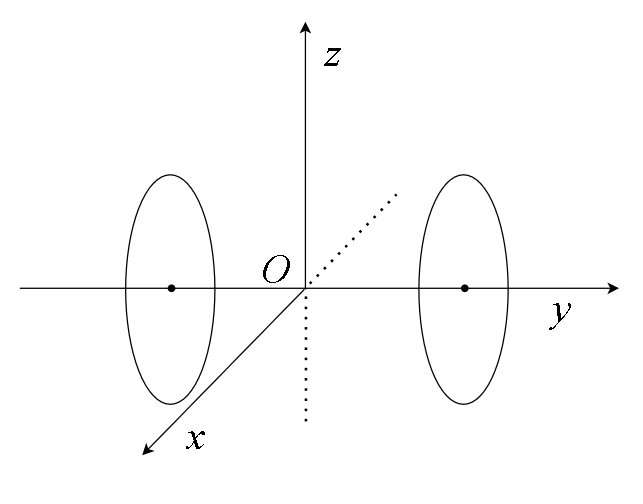
\includegraphics[scale=0.6]{./pic/坐标系.png}
    \caption{建立坐标系}
    \label{建立坐标系}
\end{figure}
建立如图\ref{建立坐标系}所示的坐标系。设单匝线圈上载有电流$I$,半径为$R$,线圈上任一电流源与圆心连线,与$x$轴正向的夹角为$\varphi$。根据对称性,我们只需要分析$yOz$平面上的一点即可。不妨设场点为$P(0,y,z)$,任一电流元$Q(R \cos \varphi,0,R \sin \varphi)$到$P$的位矢为$\bm{r}$。由几何关系可知$\bm{r}=(-R \cos \varphi,y,z-R \sin \varphi)$。根据毕奥-萨法尔定律,线圈上任一电流元在$P$点产生的磁感应强度为
\begin{equation}
    d\bm{B}=\dfrac{\mu_0}{4\pi}\dfrac{Id\bm{l}\times \bm{r}}{r^3}
\end{equation}
由于$d\bm{l}=(-R\sin \varphi d\varphi,0,R\cos \varphi d\varphi) $,所以有
\begin{equation}
    d\bm{l}\times \bm{r}
    =
    \begin{bmatrix}
       \bm{i} & \bm{j} &\bm{k}\\
       -R\sin \varphi d\varphi & 0 & R\cos \varphi d\varphi\\
       -R \cos \varphi & y & z-R \sin \varphi
    \end{bmatrix}
\end{equation}
所以在$P$点,磁感应强度的三个分量的大小为
\begin{align}
    \bm{B_x}&=\dfrac{\mu_0 IRy}{4\pi}\int_0^{2\pi} \dfrac{\cos \varphi d\varphi }{(R^2+y^2+z^2-2Rz\sin \varphi)^{3/2}} \\
    \bm{B_y}&=\dfrac{\mu_0 IRy}{4\pi}\int_0^{2\pi} \dfrac{\sin \varphi d\varphi }{(R^2+y^2+z^2-2Rz\sin \varphi)^{3/2}}  \\
    \bm{B_z}&=\dfrac{\mu_0 IR}{4\pi}\int_0^{2\pi} \dfrac{(R-z\sin \varphi)d\varphi }{(R^2+y^2+z^2-2Rz\sin \varphi)^{3/2}} 
\end{align}
可以发现,上式不能直接用初等函数表示,需要用到椭圆积分。借助文献\cite{1}可知,做变换
\begin{align}
    \theta&=\dfrac{\varphi +\pi /2}{2}\\
    r'&=\sqrt{(R+y)^2+z^2}\\
    k&=\sqrt{4Ry/r'^2},|k|<1
\end{align}
可以将磁感应强度的表达式用第一类和第二类椭圆积分表示为
\begin{align}
    \bm{B_x}&=0\\
    \bm{B_y}&=\dfrac{\mu_0 Iy}{2\pi zr'}[\dfrac{R^2+y^2+z^2}{(R-z)^2+y^2}E(k)-K(k)]\\
    \bm{B_z}&=\dfrac{\mu_0 I}{2\pi r'}[\dfrac{R^2-y^2-z^2}{(R-y)^2+z^2}E(k)+K(k)]
\end{align}
至此,我们得到了单匝线圈在轴线平面(也即全空间)的磁感应强度分布。
\subsection{对称单匝线圈的磁感应强度分布}
考虑两个单匝亥姆霍兹线圈关于原点对称分布的情况。因为磁感应强度具有矢量叠加性,因此在上一小节中推导的结论仍然适用,仅仅需要对线圈做平移变换。设两个线圈相互平行,相距为$L$,则右边线圈的磁感应强度为
\begin{align}
    B_{1z}&=\dfrac{\mu_0 I}{2\pi}\dfrac{y-0.5L}{z\sqrt{(|z|+R)^2+(y-0.5L)^2}} \cdot \\
    &[\dfrac{R^2+z^2+(y-0.5L)^2}{(|z|-R)^2+(y-0.5L)^2}E(k_1)-K(k_1)]\\
    B_{1y}&=\dfrac{\mu_0 I}{2\pi}\dfrac{1}{\sqrt{(|z|+R)^2+(y-0.5L)^2}}\cdot \\
    &[\dfrac{R^2-z^2-(y-0.5L)^2}{(|z|-R)^2+(y-0.5L)^2}E(k_1)+K(k_1)]
\end{align}
左边线圈的磁感应强度为
\begin{align}
    B_{2z}&=\dfrac{\mu_0 I}{2\pi}\dfrac{y+0.5L}{z\sqrt{(|z|+R)^2+(y+0.5L)^2}} \cdot \\
    &[\dfrac{R^2+z^2+(y+0.5L)^2}{(|z|-R)^2+(y+0.5L)^2}E(k_2)-K(k_2)]\\
    B_{2y}&=\dfrac{\mu_0 I}{2\pi}\dfrac{1}{\sqrt{(|z|+R)^2+(y+0.5L)^2}}\cdot \\
    &[\dfrac{R^2-z^2-(y-0.5L)^2}{(|z|-R)^2+(y+0.5L)^2}E(k_2)+K(k_2)]
\end{align}
其中,
\begin{align}
    k_1^2&=\dfrac{4R|z|}{(|z|+R)^2+(y-0.5L)^2}\\
    k_2^2&=\dfrac{4R|z|}{(|z|+R)^2+(y+0.5L)^2}
\end{align}
$K(k),E(k)$分别为第一类和第二类椭圆积分,即
\begin{align}
    K(k)&=\int_0^{\pi/2} \dfrac{d\varphi}{\sqrt{1-k^2 \sin ^2\varphi}}\\
    E(k)&=\int_0^{\pi/2} \sqrt{1-k^2 \sin ^2\varphi} d \varphi
\end{align}
\subsection{引入实际线圈参数}
考虑到实际线圈总是具有一定的匝数、宽度和厚度,多匝线圈不能仅仅视为多个同一位置的圆电流的叠加,而应考虑到线径对该匝线圈位置的影响。为了方便分析,假设导线按照图\ref{截面}所示的方式紧密排列。
\begin{figure}[H]
    \centering
    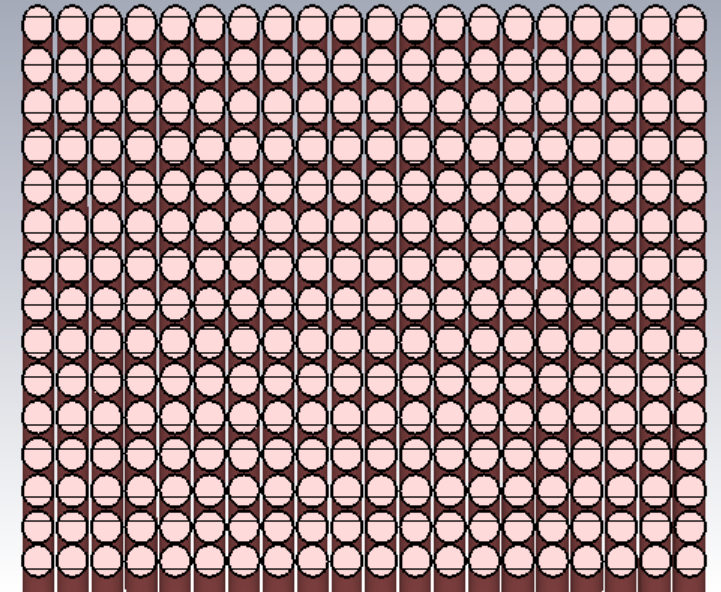
\includegraphics[width=0.4\textwidth]{./pic/线圈截面.png}
    \caption{线圈截面示意图}
    \label{截面}
\end{figure}
设线径为$d$,在$y$轴方向上线圈的匝数为$n_1$,在$z$轴方向上线圈的匝数为$n_2$。将单匝线圈视为集中在中心环线上的圆电流,则$L,R$应该做如下修正
\begin{align}
    L'&=L'(m,n)=[\dfrac{1}{2}L+(n-\dfrac{n_1}{2}+\dfrac{1}{2})d]\times 2\\
    R'&=R'(m,n)=R+(m-\dfrac{n_2}{2}+\dfrac{1}{2})d
\end{align}

其中,$n,m$分别用于线圈计数,$n=0,1,2,\cdots n_1-1,m=0,1,2,\cdots n_2-1$,且$n=m=0$代表$|y|$坐标和实际半径最小的那一匝线圈。
上节关于椭圆积分的公式需要修正为
\begin{align}
    k_1^2&=\dfrac{2L'(m,n)|z|}{(|z|+\dfrac{1}{2}L'(m,n))^2+(z-\dfrac{1}{2}L+R'(m,n))^2}\\
    k_2^2&=\dfrac{2L'(m,n)|z|}{(|z|+\dfrac{1}{2}L'(m,n))^2+(z+\dfrac{1}{2}L+R'(m,n))^2}\\
    B_{1z}&=\dfrac{\mu_0 I}{2\pi}\dfrac{y-0.5L'}{z\sqrt{(|z|+R')^2+(y-0.5L')^2}} \cdot \\
    &[\dfrac{R'^2+z^2+(y-0.5L')^2}{(|z|-R')^2+(y-0.5L')^2}E(k_1)-K(k_1)]\\
    B_{1y}&=\dfrac{\mu_0 I}{2\pi}\dfrac{1}{\sqrt{(|z|+R')^2+(y-0.5L')^2}}\cdot \\
    &[\dfrac{R'^2-z^2-(y-0.5L')^2}{(|z|-R')^2+(y-0.5L)^2}E(k_1)+K(k_1)]\\
    B_{2z}&=\dfrac{\mu_0 I}{2\pi}\dfrac{y+0.5L'}{z\sqrt{(|z|+R')^2+(y+0.5L')^2}} \cdot \\
    &[\dfrac{R'^2+z^2+(y+0.5L')^2}{(|z|-R')^2+(y+0.5L')^2}E(k_2)-K(k_2)]\\
    B_{2y}&=\dfrac{\mu_0 I}{2\pi}\dfrac{1}{\sqrt{(|z|+R')^2+(y+0.5L')^2}}\cdot \\
    &[\dfrac{R'^2-z^2-(y+0.5L')^2}{(|z|-R')^2+(y+0.5L)^2}E(k_2)+K(k_2)]
\end{align}
\section{实物测试}
由于实验室线圈已经封装,不便拆开测量线径、厚度和宽度,故不可能通过理论计算直接得到与实验值接近的计算结果。为了检验模型的正确性,我们采用参数拟合的方法,即先测量得出实验值,将线径、厚度和宽度作为参数代入理论模型进行优化计算。如果能够得到一组参数,使得在该参数条件下理论模型与实测值的误差在允许范围内,同样可以说明模型有效。
\subsection{实验方案}
现利用实验室已有的设备测量亥姆霍兹线圈的磁场分布。由于装置的对称性,只需要测量轴线平面上的磁场分布即可。实验仪器采用霍尔效应测量磁场强度,只能检测垂直于霍尔导体某一面的磁感应强度,即本文坐标系下$y$轴方向上的磁感应强度。设定霍尔工作电流为5mA;两线圈串联,励磁电流为0.5A。探头可以在$x$轴和$y$轴方向上移动。实验步骤如下
\begin{enumerate}
    \item 将两线圈的距离设定为$L=2R$,将探头所在金属棒对应的刻度线与零刻度线对齐。
    \item 将探头的$x$坐标设置为0。
    \item 向线圈通电。
    \item 在$y$轴方向上移动探头,使其从$y=-19cm$到$y=+19cm$范围内变化,每经过一个位置记录下对应点的霍尔电压。在特殊位置,如线圈所在位置、两线圈连线中点等处适当增加取点个数。
    \item 测完一组数据后,改变探头的$x$坐标,在$x=2,4,6,8cm$处重复上面的测量过程。
    \item 改变两线圈的位置,在距离为$L=R,0.5R$时重复上述测量过程。
\end{enumerate}
如图是实验装置的实物图
\begin{figure}[H]
    \centering
    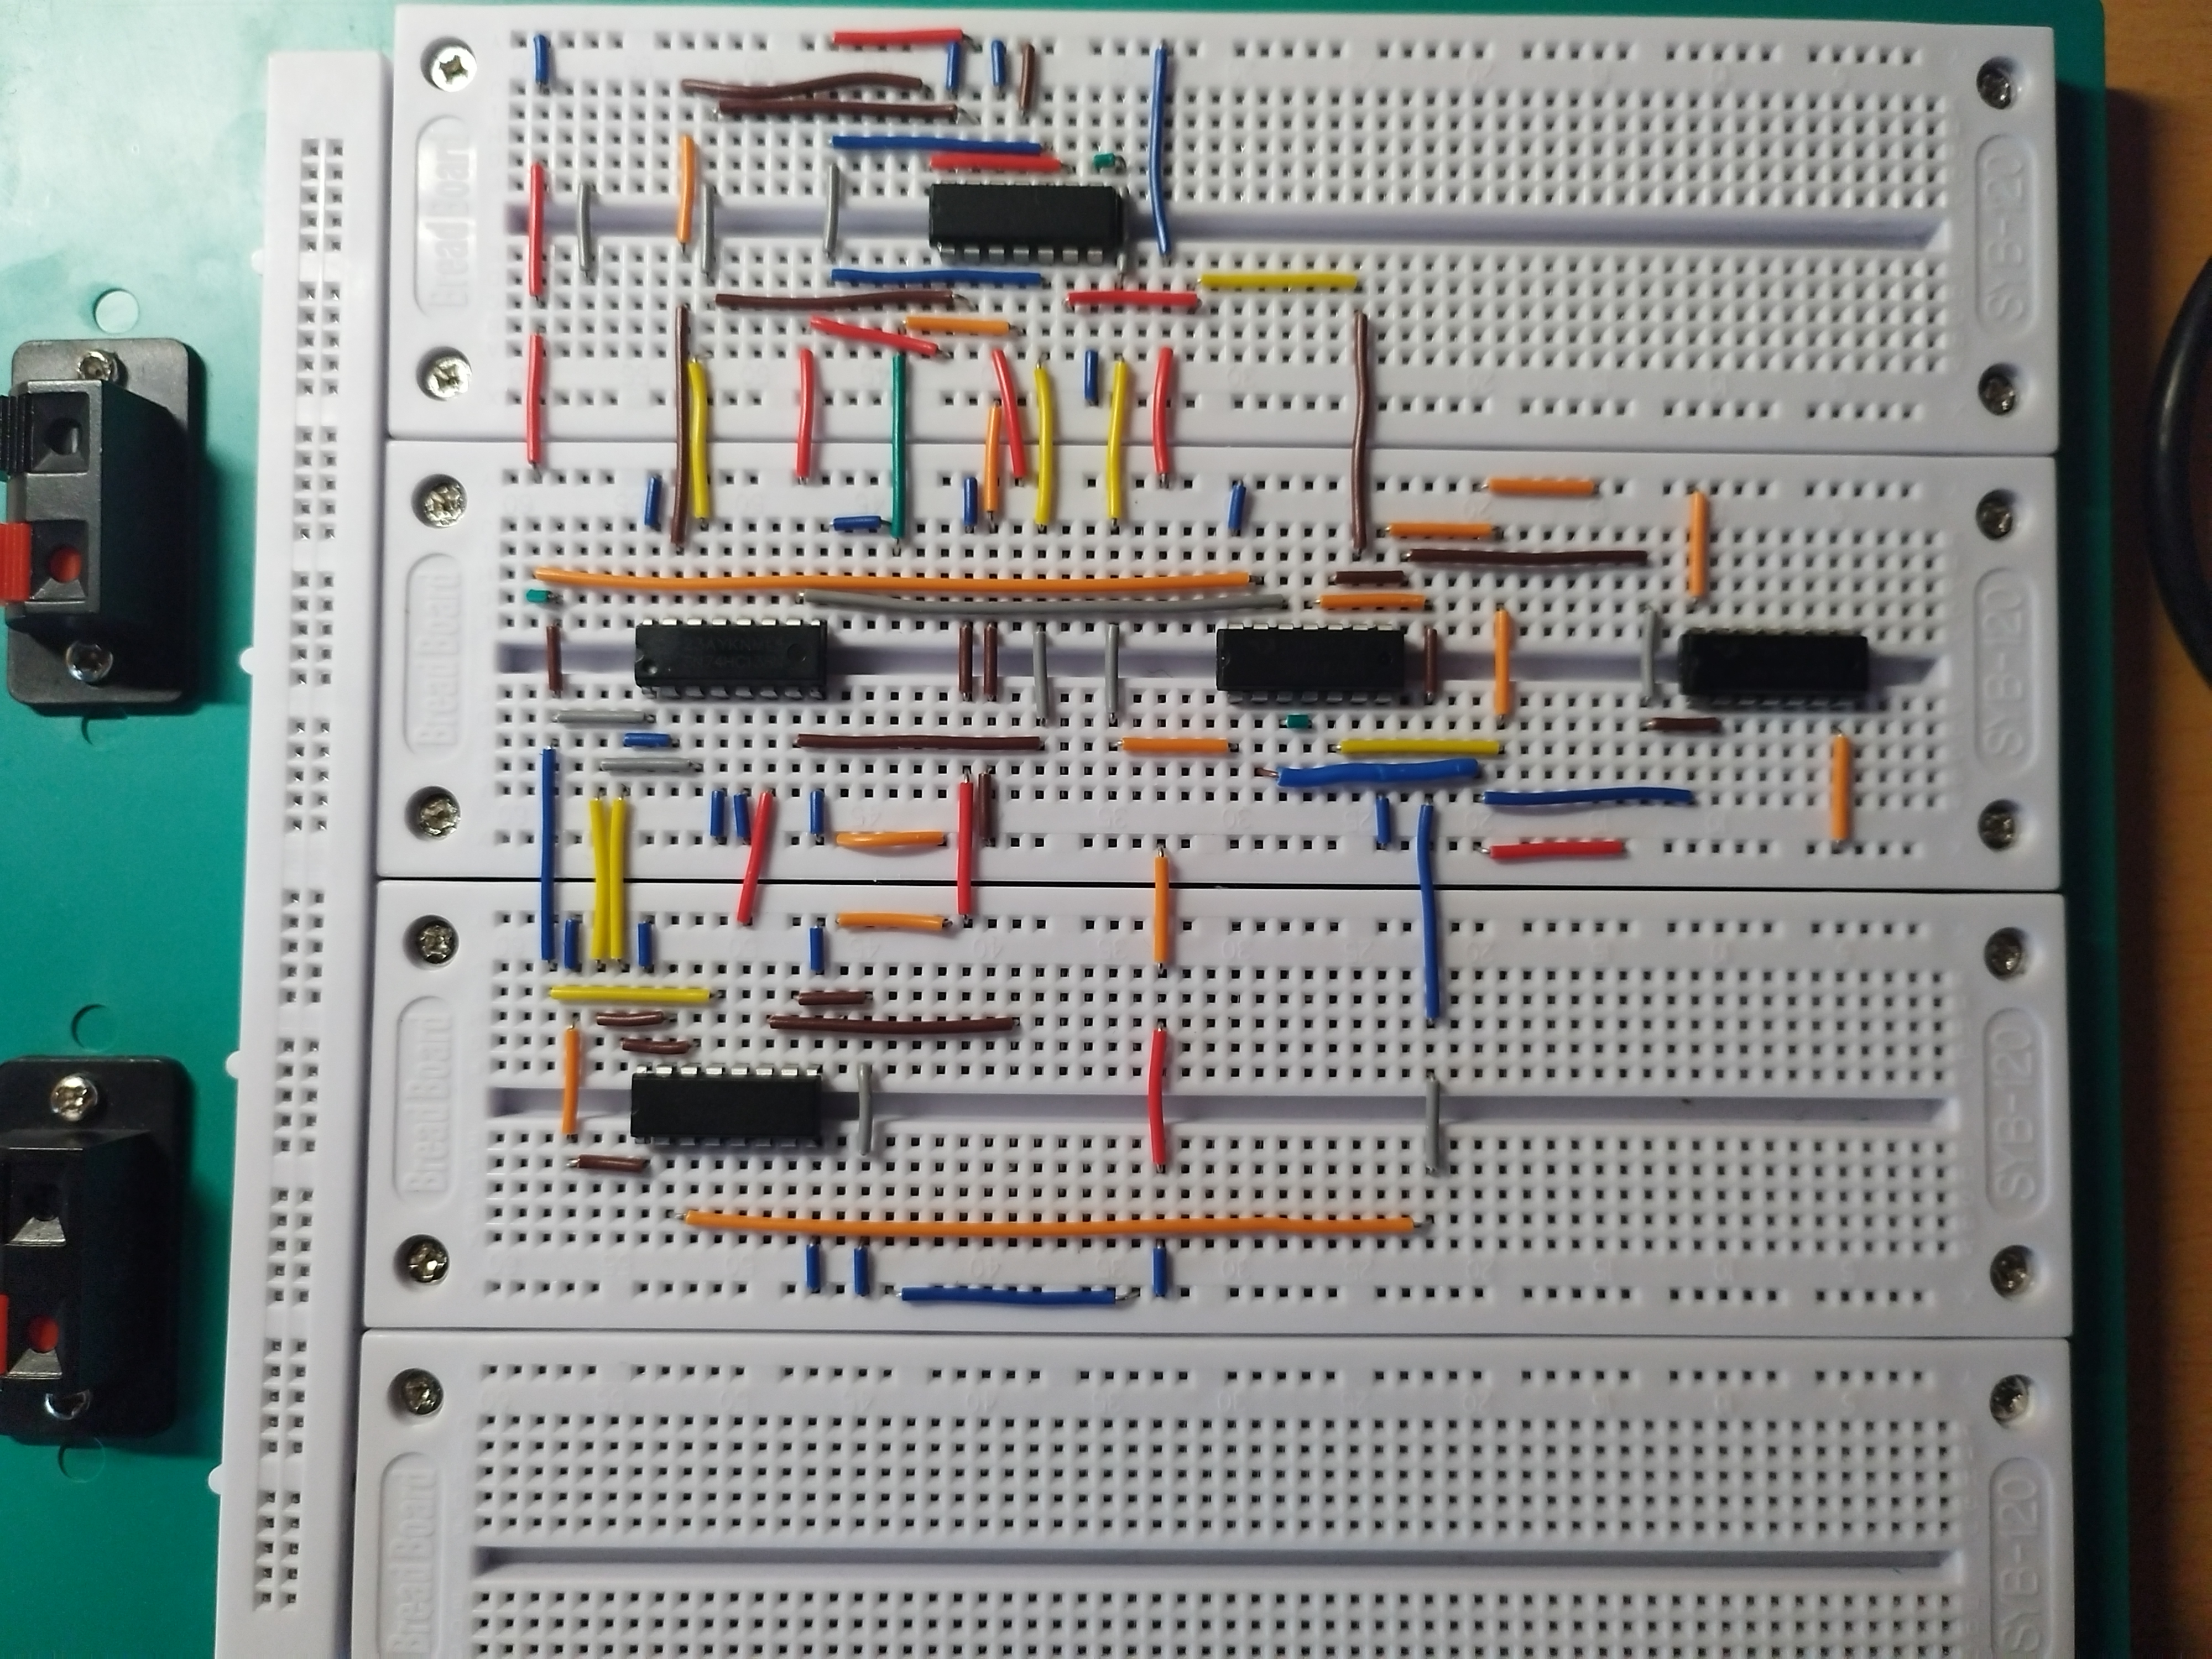
\includegraphics[width=0.4\textwidth]{./pic/实物图.jpg}
    \caption{实验装置图}
    \label{截面}
\end{figure}
\subsection{实验数据处理}
按照上述实验方案采集数据,得到的实验数据部分如表\ref{实验数据}所示
\begin{table}[H]
    \centering
    \caption{$L=2R$时的实验数据(部分)}
    \begin{tabular}{cccc}
        \hline
        $y(x=2)$cm & $U_H$/mV & $y(x=4)$ cm& $U_H$/mV \\ \hline
        -19 & 0.64 & -19&	0.58\\
        -18	&0.75&	-18	&0.67\\
        $\cdots$ &$\cdots$ &$\cdots$ &$\cdots$\\
        -0.3 &	0.9	&-0.3	&0.89\\
        0	&0.92	&0	&0.89\\
        0.3	&0.91	&0.3&	0.89\\
        $\cdots$ &$\cdots$ &$\cdots$ &$\cdots$\\
        18&	0.65	&18	&0.64\\
        19&	0.56	&19&	0.55\\ \hline
    \end{tabular}
    \label{实验数据}   
\end{table}
根据霍尔电压的计算公式
\begin{equation}
    U_H=K_HIB
\end{equation}
可以反解出磁感应强度$B$。借助Matlab处理实验数据并作图,可以看出$y$轴方向上磁场分量的分布情况。如图\ref{实测surf}到图\ref{实测surf2}是$L=2R,R,0.5R$的磁场分布图,可以看到当$L=R$时,两线圈之间的区域有较为平坦的匀强磁场区,但是偏离轴线的程度越大,均匀性越差。
\begin{figure}[H]
    \centering
    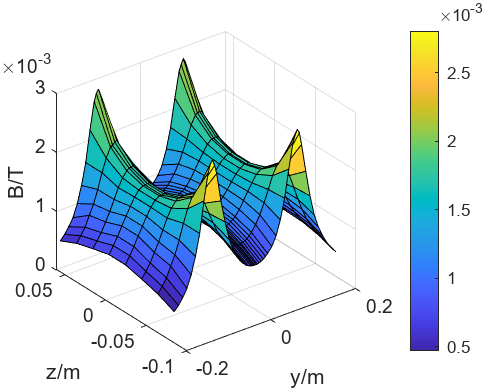
\includegraphics[scale=1]{./pic/realsurf2R.png}
    \caption{$L=2R$时的磁场分布曲面图} 
    \label{实测surf}
\end{figure}
\begin{figure}[H]
    \centering
    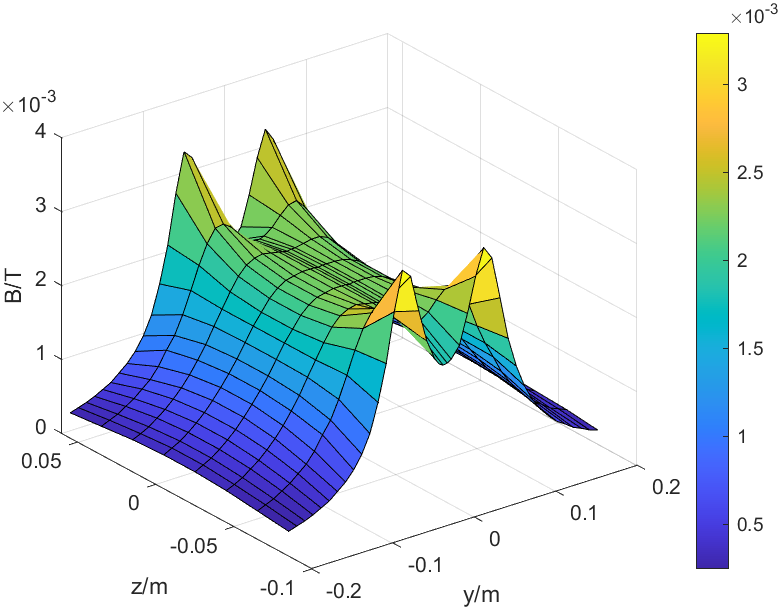
\includegraphics[scale=0.6]{./pic/realsurfR.png}
    \caption{$L=R$时的磁场分布曲面图} 
\end{figure}
\begin{figure}[H]
    \centering
    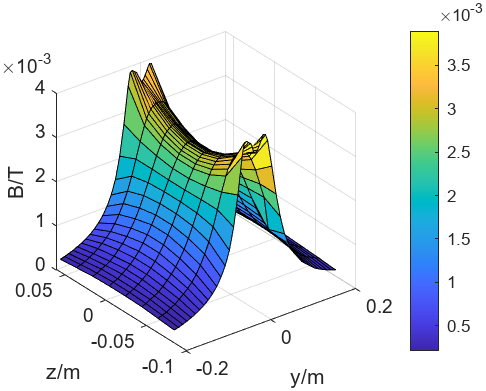
\includegraphics[scale=1]{./pic/realsurf0.5R.png}
    \caption{$L=0.5R$时的磁场分布曲面图} 
    \label{实测surf2}
\end{figure}
\subsection{模型检验}
在实验中和在理论模型中,我们得到了两个关于磁感应强度的二元函数曲面。记理论模型得到的函数为$B(y,z)$。其上任一点的坐标为$y,z$轴坐标,函数值为该点磁感应强度在$y$轴方向上的分量。为了检验理论模型与实际测量值的吻合度,我们求出两个曲面上坐标相同的两个点的曼哈顿距离,即函数值与实测值之差的绝对值:
\begin{equation}
    D(y,z)=|B(y,z)-B_0(y,z)|
\end{equation}
其中$B_0(y,z)$是该点的实测值。
建立函数
\begin{equation}
    f=\sum_{y} \sum_{z} D(y,z)
\end{equation}
将线圈的匝数、宽度、厚度作为参变量代入上式计算,若能找到一组参数组合,能使$f$达到最小值且该最小值足够小,则认为模型与实际情况吻合较好。

利用Matlab的优化工具箱,使用fmincon方法,把$f$作为待求最小值的函数,把匝数、宽度、厚度作为变量,发现该方法收敛速度很快,极易陷入局部最优解。为此,换用全局优化工具箱,使用遗传算法,将$f$作为适应度函数,线圈参数视为“基因”。在有限次迭代后,发现$f$能够收敛在一个极小值附近。更改初始值,优化得到的线圈参数几乎不变,说明该解的稳定性较好。表\ref{不同情况下线圈匝数的解}列出了不同情况下线圈匝数的解
\begin{table}[H]
    \centering
    \caption{不同情况下线圈参数的解}
    \begin{tabular}{cccc}
        \hline
        线圈距离 & $d$/m & $n_1$/匝 & $n_2$/匝\\ \hline
        $L=2R$ & 0.0009 & 21.7733 & 22.3475\\
        $L=R$ &0.0007  & 21.8547  & 22.4576\\
        $L=0.5R$ &0.0009 &21.6759 &22.1964\\
        平均值 & 0.0008&21.7680& 22.3338 \\ \hline
    \end{tabular}
    \label{不同情况下线圈匝数的解}   
\end{table}
将该解视作线圈实际参数带入计算式求解理论值与实际值的距离,平均每点的绝对误差如表所示
\begin{table}[H]
    \centering
    \caption{理论值与实测值的平均绝对误差}
    \begin{tabular}{cccc}
        \hline
        $L=2R$ & $L=R$ & $L=0.5R$ & 平均值\\ \hline
        $8.25\times 10^{-5}$ & $8.66\times 10^{-5}$ & $1.00\times 10^{-4}$ 
         & $8.98\times 10^{-5}$  \\ \hline
    \end{tabular}
    \label{每个场点处的平均百分误差}   
\end{table}

综上所述,该模型与实际情况较为吻合。如图\ref{matlab理论surf}到图\ref{matlab理论surf2}是将线圈参数代入理论模型计算出的磁场分布曲面图
\begin{figure}[H]
    \centering
    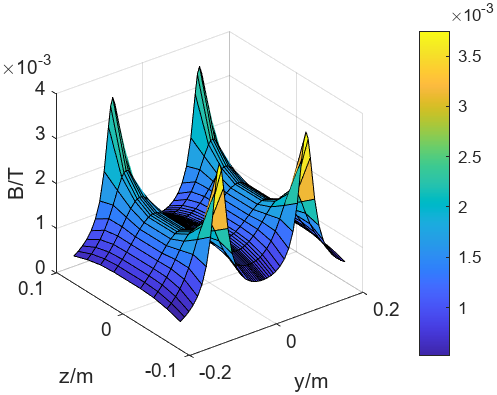
\includegraphics[scale=1]{./pic/matlab2R.png}       
    \caption{$L=2R$时的磁场分布曲面图} 
    \label{matlab理论surf}
\end{figure}
\begin{figure}[H]
    \centering
    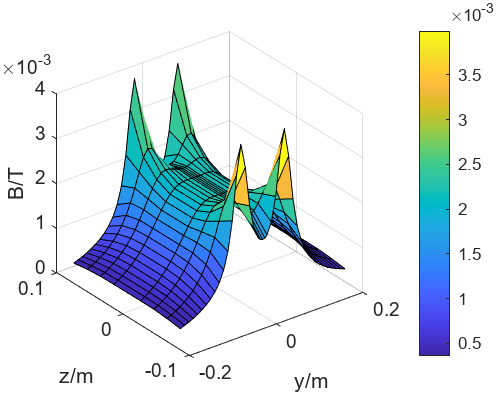
\includegraphics[scale=1]{./pic/matlabR.png}
    \caption{$L=R$时的磁场分布曲面图} 
\end{figure}
\begin{figure}[H]
    \centering
    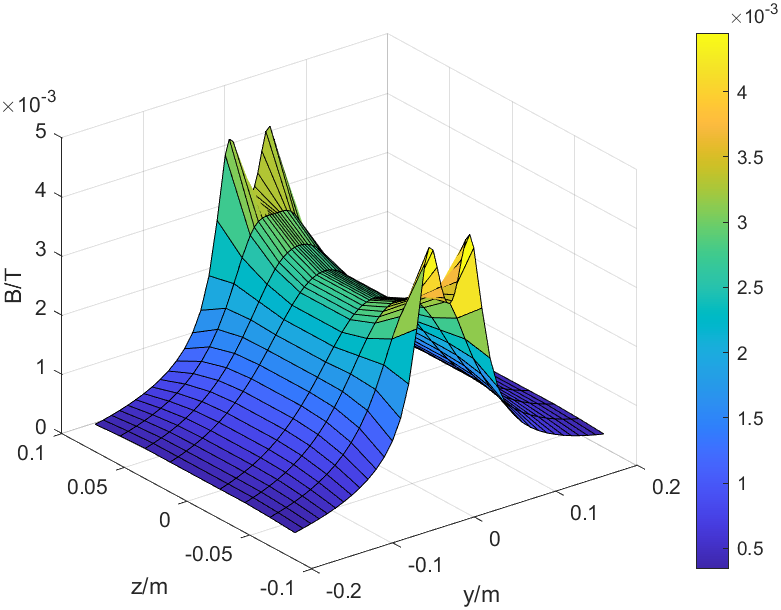
\includegraphics[scale=0.6]{./pic/matlab0.5R.png}
    \caption{$L=0.5R$时的磁场分布曲面图} 
    \label{matlab理论surf2}
\end{figure}
\section{仿真测试}
上述实验验证基本验证了理论模型的正确性,但是仍有不足:
\begin{enumerate}
    \item 实验只检验了一个方向上的磁感应强度分量,并没有检验其他分量。
    \item 受限于实验装置,只能测量线圈内部和周围一小片区域的磁场,对于较大范围内模型的正确性仍有待检验。
\end{enumerate}
为此,我们利用电磁仿真软件CST来弥补上述不足。本文采用的软件为CST Studio Suite 2021版,内置了亥姆霍兹线圈的仿真模板,可以方便地为模型检验提供帮助。按照图\ref{截面}的假设构建模型,设置线圈位置、励磁电流,并将匝数等作为参数进行扫描,得到磁场的空间分布。如图是$L=2R$时的三维磁场矢量图。
\begin{figure}[H]
    \centering
    \includegraphics[scale=0.5]{./pic/vector.bmp}
    \caption{$L=2R$时的三维磁场矢量图}
    \label{三维磁场矢量图}
\end{figure}
为了检验理论模型,单独分析该结果的$y$方向和$z$方向分量。沿用上文曼哈顿距离的计算方法,算出理论模型与仿真值在每个场点处的平均绝对误差如表\ref{每个场点处的平均百分误差}所示
\begin{table}[H]
    \centering
    \caption{平均绝对误差}
    \begin{tabular}{ccc}
        \hline
        线圈距离 & $y$轴方向($10^{-4}$) & $z$轴方向($10^{-4}$) \\ \hline
        $L=2R$ & 9.8323 & 8.8237 \\
        $L=R$ & 6.5569  & 6.7501  \\
        $L=0.5R$ & 7.4316 &5.7452 \\
        平均值 & 7.9403& 7.1063 \\ \hline
    \end{tabular}
    \label{每个场点处的平均百分误差}   
\end{table}

说明理论模型与仿真结果近似。如图\ref{$L=2R$时的$y$轴方向磁感应强度的分量示意图}是利用仿真软件得到的$y$轴方向磁场分量图。
\begin{figure}[H]
    \centering
    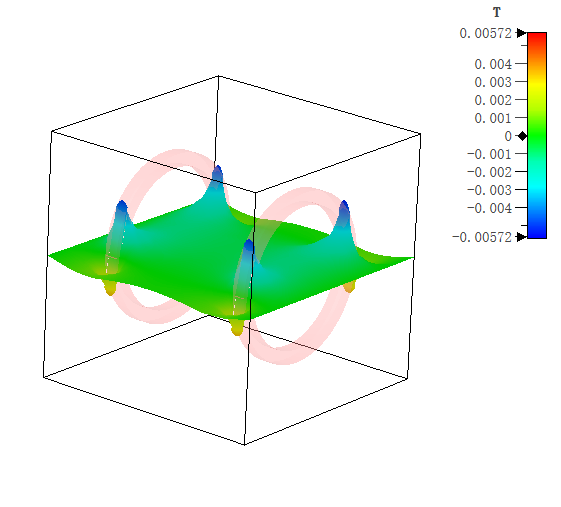
\includegraphics[scale=0.5]{./pic/L=2R仿真.png}
    \caption{$L=2R$时的$y$轴方向磁感应强度的分量示意图}
    \label{$L=2R$时的$y$轴方向磁感应强度的分量示意图}
\end{figure}
\begin{thebibliography}{4}
    \bibitem{zhuping}朱平.圆电流空间磁场分布[J].大学物理,2005,(09):13-17.DOI:10.16854/j.cnki.1000-0712.2005.09.005
    \bibitem{pengzhonghan}彭中汉.亥姆霍兹线圈的均匀磁场区[J].大学物理,1985,(05):13-16.DOI:10.16854/j.cnki.1000-0712.1985.05.005        
    \bibitem{moyunfei}莫云飞,周群益,侯兆阳等.亥姆霍兹线圈磁场均匀范围的研究[J].大学物理,2021,40(02):18-20+35.DOI:10.16854/j.cnki.1000-0712.200137
    \bibitem{1}刘保义,张明霞.圆环电流在全空间形成的磁感应强度分布[J].天水师范学院学报,2009,29(02):65-66.
\end{thebibliography}
\end{multicols}
\end{document}
